

\section{Принцип максимума для уравнения теплопроводности. Теорема о единственности решения задачи Коши уравнения теплопроводности в классе $\mathbf{M_2(T)}$ (без доказательства) }
%Никитушка отмочил красоту
$\bullet$ Пусть $\Omega$ - ограниченная область в $\R^n$, T > 0, 
$Q_T = (0,T) \times \Omega$ - цилиндр. Сечение цилиндра плоскостью $t = \tau$ обозначим $\Omega_\tau$

\begin{definition}
{\bf Параболическая граница области $Q_T$} - множество $\Gamma_T = \Omega_0 \cup \{[0,T] \times \partial{\Omega} \}$
\end{definition}
\begin{center}
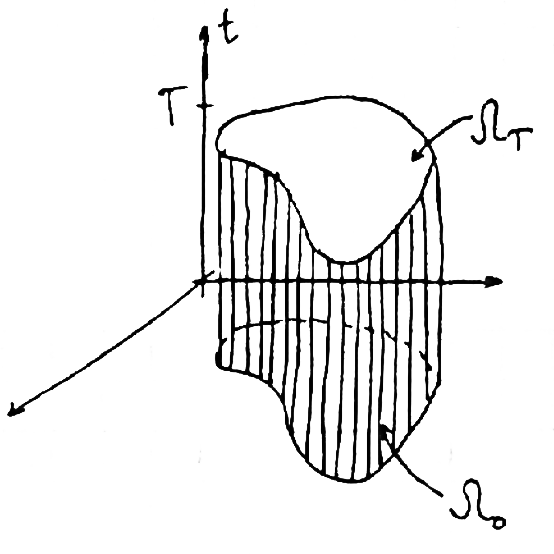
\includegraphics[scale=0.5]{11_1_new}
\end{center}

Определим оператор $\mathrm{L} : \mathrm{L}u(t,x) = u_t - a^2 \Delta_xu$, где 
$u \in C_{t, x}^{1,2}(Q_T)$

\begin{theorem}

{\bf (Принцип максимума)} Пусть $u(t,x) \in C_{t, x}^{1,2}(Q_T) \cap C(\overline{Q_T})$, и пусть 
$\mathrm{L}u(t,x) \leq 0$ в $Q_T$. Тогда $\max\limits_{(x,t) \in \overline{Q_T}} u(t,x)$ достигается на параболической границе $ \Gamma_T $ области $Q_T$


\begin{proof}
Возьмем усеченный цилиндр $Q_{T-\delta}$. Рассматриваются $M = \max\limits_{\overline{Q_{T-\delta}}} u(t,x)$ и $m = \max\limits_{\Gamma_{T-\delta}} u(t,x)$. Теорема утверждает, что $M$ не превосходит $m$.\\
\begin{itemize}
\item {\bf Пусть это не так} и $m < M$. Тогда $\exists (t^1,x^1) \in Q_{T-\delta} \cup \Omega_{T-\delta}$ такая, что $M = u(t^1, x^1)$. \\
Т.к. это точка максимума гладкой функции, $u_{x_ix_i}(t^1,x^1) \leq 0$, а $u_t(t^1, x^1) \geq 0$ (Если внутри, то равенство, если на верхней кромке, то $\geq 0$).\\
Значит, значение образа $u(t,x)$ под действием оператора $\mathrm{L}$ в точке $(t^1, x^1): \boxed{\mathrm{L}u(t^1, x^1) = u_t -a^2 \Delta_x \eval{u}_{(t^1,x^1)}  \geq 0}$.\\
Для противоречия необходимо показать, что неравенство строгое.\\

 й\item {\bf Строгость:}
Возьмем функцию $v_\beta(t,x) = u(t,x) +\beta \abs*{x-x^1}^2, \beta = \dfrac{M-m}{2(\mathrm{diam} Q_T)^2}$ - такая же гладкая, как $u$.\\
 На параболической границе $v_\beta \leq m + \frac{M-m}{2d^2}\cdot d^2 = \frac{M+m}{2} < M$.
Тем не менее, $v_\beta(t^1, x^1) = M \Rightarrow$ максимум $v_\beta$ - не на параболической границе.\\
Пусть он в точке $(t^2, x^2) \notin \Gamma_{T-\delta}$. Тогда $\mathrm{L}\eval*{v_\beta}_{(t^2,x^2)} = \mathrm{L}\eval{u}_{(t_2, x_2)} - \beta d^2 2n \boxed{\geqslant} 0 \Rightarrow \mathrm{L}\eval{u}_
{(t_2,x_2)} {\geq} \beta d^2 2n > 0 \Rightarrow$ {\bf Противорчие} (вывод $\boxed{\geq}$ аналогичен рамке выше)
 
\item {\bf Предельный переход с $\delta \rightarrow+0$:}
Пусть $u_{*} = \max\limits_{\Gamma_T} u(t,x)$. \\
Тогда $\max\limits_{\overline{Q_{T-\delta}}}u(t,x) \leq \max\limits_{{\Gamma_{T-\delta}}}u(t,x) \leq \max\limits_{{\Gamma_{T}}}u(t,x) = u_* \Rightarrow
u(t,x) \leq u_*$
во всех точках $\overline{Q_T} \diagdown \Omega_T$\\
$\eval{u(t,x)}_{\Omega_T} = \lim\limits_{(\widehat{t}, \widehat{x}) \in Q_T \rightarrow (t,x) \in \Omega_T} u(\widehat{t},\widehat{x}) \boxed{\leq} u_*$ 
\\($\boxed{\leq}$ - предельный переход в неравенствах.) Теорема доказана.
\end{itemize}

\end{proof}
\end{theorem}


\begin{conseq}
Пусть $u(t,x) \in C^{1,2}_{t,x}(Q_T) \cap C(\overline{Q_T}), \mathrm{L}u = 0 \Forall(t,x) \in Q_T$.
 Тогда $\max\limits_{\overline{Q_T}}u(t,x)$ и $\min\limits_{\overline{Q_T}}u(t,x)$ достигаются на параболической границе $\Gamma_T$ множества $Q_T$
 \begin{proof}
 Максимум достигается,т.к. $\mathrm{L}u \leq 0$, минимум достигается, т.к. $\mathrm{L}(-u) \leq 0$
 \end{proof}
\end{conseq}


{\bf Единственность решения задачи Коши}\\
Вообще говоря, решение единственным будет не всегда. Но если
 ограничиться некоторым классом функций, то в нем решение может
  оказаться единственным. Введем такой класс.\\
  
  
\begin{itemize}
\item Пусть $T > 0, \sigma \geq 0$. {\bf Слой толщины T} - множество $\Pi_T =\brk[c]*{(t,x): 0 < t < T; x \in \R^n}$\\
Обозначим $M_\sigma(T)$ -{\bf класс функций} $u(t,x) \in C^{1,2}_{t,x}(\Pi_T) \cap
C(\overline{\Pi_T})$ таких, что $\forall\: u(t,x) \Exists A > 0 , \alpha \geq 0$ такие,
что $\abs*{u(t,x)} \leq A\exp^{\alpha \abs*{x}^{\sigma}} \Forall (t,x) \in \overline{\Pi_T}$


\begin{lemma}
$M_\sigma(T)$ - линейное пространство, причем 
$\sigma_0 \leq \sigma_1 \Rightarrow M_{\sigma_0}(T) \subset M_{\sigma_1}(T)$
\begin{proof}
Очевидно.
\end{proof}
\end{lemma}

\begin{lemma}
$\forall T > 0$ функция $u_T(t,x) = \dfrac{1}{(T-t)^{\frac{n}{2}}}
\exp^{\dfrac{\abs*{x}^2}{4a^2(T-t)}}, t<T, x \in \R^n$ удовлетворяет
 однородному уравнению теплопроводности
\begin{proof}
\begin{itemize}

\item $u_T \in C^\infty \brk[c]*{t<T, x \in \R^n}$

\item $\pd{u_T}{t} = \brk[s]*{\dfrac{n}{2(T-t)^\frac{n}{2}} + \dfrac{1}{(T-
t)^{\frac{n}{2}}}{\dfrac{\abs*{x}^2}{4a^2(T-t)^2}}}
\exp^{\dfrac{\abs*{x}^2}{4a^2(T-t)}}$

\item $\Delta_xu_T = \brk[s]*{\dfrac{1}{(T-t)^\frac{n}
{2}}\dfrac{2n}{4a^2(T-t)} + \dfrac{1}{(T-t)^\frac{n}
{2}}\dfrac{4\abs*{x}^2}{4^2a^4(T-t)^{2}}}
\exp^{\dfrac{\abs*{x}^2}{4a^2(T-t)}} \Rightarrow 
(u_T)^{'}_t - a^2 \Delta_x u_T = 0$ ч.т.д
\end{itemize}
\end{proof}
\end{lemma}


\item {\bf Класс Тихонова} - $M_2(T)$

\begin{lemma}
Пусть $v(t,x)$ такова, что $v \in M_2(T)$ и $v$ - решение полностью 
однородной ЗК $\brk[c]*{\mathrm{L}v = 0, \eval{v}_{t=0}}$.
Тогда $\exists T_1 \leq T: \abs*{v} \leq \varepsilon u_{2T_1}(x,t) \Forall \varepsilon > 0$

\begin{proof}
$\abs*{v} \leq A \exp^{\alpha \abs*{x}^2} \Forall t, x \in
 \overline{\Pi_T}$. Выбираем $T_1 \leq T: \dfrac{1}{8a^2T_1} >
 \alpha : T_1 = \min\brk[c]*{T, \dfrac{1}{16\alpha a^2}}$\\
 Возьмем $\varepsilon > 0$ и $\omega_e^{\pm}(t,x) = \varepsilon
 u_{2T_1} \pm v(t,x)$. 
 Нужно показать, что $\omega_e^{\pm}(t,x) > 0$:\\
 
 $
 \omega_e^{\pm}(t,x) \geq \varepsilon u_{2T_1} - \abs*{v(t,x)} \geq \varepsilon  u_{2T_1}
  - A\exp^{\alpha \abs*{x}^2} = 
  \dfrac{\varepsilon}{(2T_1-t)^{\frac{n}{2}}}\exp^{\dfrac{\abs*{x}^2}{4a^2(2T_1-t)}} - A\exp^{\alpha \abs*{x}^2}
  \geq
   \dfrac{\varepsilon}{(2T_1-t)^{\frac{n}{2}}}
  \exp^{\dfrac{\abs*{x}^2}{4a^2 2(T_1)}} - A\exp^{\alpha \abs*{x}^2}=
   \dfrac{\varepsilon}{(2T_1)^{\frac{n}{2}}}
   \exp^{\dfrac{\abs*{x}^2}{8a^2(T_1)}}
   \brk[s]*{1 - 
      \boxed{  
      \dfrac{(2T_1)^{\frac{n}{2}}}{\varepsilon}A 
      \exp^{-\brk*{\frac{1}{8a^2(T_1)}-\alpha}\abs*{x}^2}}  
      }
 $\\
 (для выделенной части $\exists R>0:$ эта часть $<\frac{1}{2}$ при 
 $\abs*{x} > R$)\\
Значит, $\forall (t,x) : 0 \leq t \leq T$ и $\abs*{x} \geq R \ \Rightarrow\omega_e^{\pm}(t,x)>0$.
\begin{center}
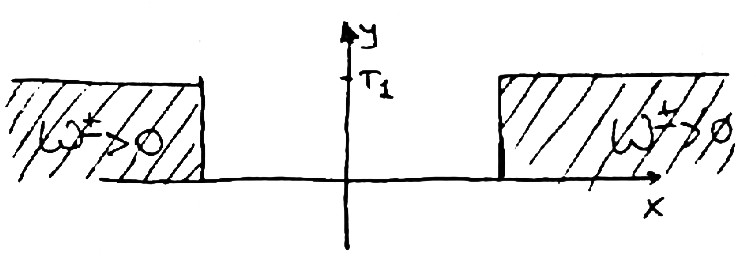
\includegraphics[scale=0.5]{11_2_new}
\end{center}
Но $\omega_e^{\pm}(t,x)$ удовлетворяет уровнению теплопроводности $\Rightarrow$ на $\Gamma_{T_1}$ достигаются максимум и минимум 
$\omega_e^{\pm}(t,x) \Rightarrow$ он строго $>0 \Rightarrow \omega_e^{\pm}(t,x)>0$ всюду в полосе $(0,T_1)$.
Итак,$\mp v(t,x) \leq \varepsilon u_{2T_1}(t,x) \Rightarrow \abs*{v} \leq \varepsilon u_{2T_1}(t,x) \Forall \varepsilon > 0 \Rightarrow v\equiv 0$ в $\overline{\Pi_{T_1}}$
 
\end{proof}
\end{lemma}

\begin{theorem}
Задача Коши $\mathrm{L}u = f(x,t), \eval{u}_{t = 0} = u_0(x)$ в {\bf классе Тихонова} не может иметь более одного решения в полосе $\Pi_T$

\begin{proof}
Пусть существует два решения: $u_1$ и $u_2$. Возьмем $v(t,x) = u_2 - u_1$. Функция $v$ удовлетворяет полностью однородной ЗК и лежит в {\bf классе Тихонова} 
$\Rightarrow$ в полосе $\Pi_{T_1}$, где $T_1$ определенно из предыдущей леммы, будет $v\equiv 0$\\
Если $T \leq T_1$, то все доказано. В противном случае вводим:\\
$w(t,x) = v(t+T_1,x)$. Она удовлеворяет:
  \begin{equation}
  \begin{cases}
  & w_t - a^2\Delta_xw=0\\
  &\eval{w}_{t=0} = 0, T_1 \leq t < T,x \in \R^n
  \end{cases}
  \end{equation}
$\Rightarrow$ в полосе $(0,T_1)$ получим $w \equiv 0$\\
($T_1$ определяется $\dfrac{1}{8a^2\alpha} \Rightarrow$ одно и то же)\\
Так за конечное число шагов $N = \lceil{\frac{T}{T_1}} \rceil$ мы покроем всю $\Pi_T$
\end{proof} 
\end{theorem}


\end{itemize}



